\documentclass[11pt]{article}
\usepackage[letterpaper,left=1.05in,right=1.05in,top=0.90in,bottom=0.90in]{geometry}
\usepackage{mathptmx}
\usepackage{amsmath,amssymb}
\usepackage{booktabs}
\usepackage{threeparttable}
\usepackage{graphicx}
\usepackage{setspace}
\usepackage{caption}
\usepackage{microtype}
\usepackage{titlesec}
\usepackage{natbib}
\usepackage{xcolor}
\usepackage{enumitem}
\usepackage{float}
\usepackage{array}
\usepackage[colorlinks=true,linkcolor=blue!55!black,citecolor=blue!55!black,urlcolor=blue!55!black]{hyperref}

\hypersetup{
  pdftitle={Climate Risk and Business Development Companies: Replication, Factor Maintenance, and Regulatory Capacity},
  pdfauthor={Yirui Mai},
  pdfsubject={CRISK replication and business development companies},
  pdfkeywords={climate risk, CRISK, business development companies, private credit, asset coverage}
}

\setstretch{1.28}
\setlength{\parindent}{0.24in}
\setlength{\parskip}{0pt}
\setlength{\bibsep}{3pt}
\titleformat{\section}{\large\bfseries}{\thesection}{0.65em}{}
\titleformat{\subsection}{\normalsize\bfseries}{\thesubsection}{0.60em}{}
\titlespacing*{\section}{0pt}{1.45em}{0.62em}
\titlespacing*{\subsection}{0pt}{1.05em}{0.42em}
\captionsetup{font=small,labelfont=bf,labelsep=period,justification=justified,singlelinecheck=false}
\pagestyle{plain}
\makeatletter
\setlength{\@fptop}{0pt}
\setlength{\@fpsep}{12pt plus 1fil}
\setlength{\@fpbot}{0pt plus 1fil}
\makeatother

\newcommand{\CRISK}{\mathrm{CRISK}}
\newcommand{\LRMES}{\mathrm{LRMES}}
\newcommand{\figref}[1]{\hyperref[#1]{Figure~\ref*{#1}}}
\newcommand{\tabref}[1]{\hyperref[#1]{Table~\ref*{#1}}}
\newcommand{\appref}[1]{\hyperref[#1]{Appendix~\ref*{#1}}}

\begin{document}
\pagenumbering{gobble}

\begin{titlepage}
\thispagestyle{empty}
\centering
\vspace*{0.42in}
{\LARGE\bfseries Climate Risk and Business Development Companies:\\[0.10in]
Replication, Factor Maintenance, and Regulatory Capacity\par}
\vspace{0.34in}
{\large Yirui Mai\par}
\vspace{0.07in}
{\normalsize Baruch College, City University of New York\par}
\vspace{0.17in}
{\normalsize August 2026\par}

\vfill
\begin{minipage}{0.86\textwidth}
\noindent\textbf{Abstract.}
This paper replicates CRISK for ten large U.S. banks and extends its market-based stress mechanism to business development companies (BDCs). Mean bank climate beta rises by 0.230 in 2020 (standard error 0.029), all ten banks move in the predicted direction, and replicated top-four marginal CRISK and signed CRISK increases recover 85.3 and 86.5 percent of published magnitudes. The high-frequency maximum, however, follows the November vaccine/value rotation rather than the March oil-price break. The published post-KOL fixed basket tracks KOL at 0.454 daily and 0.832 weekly; the associated BDC exposure coefficient rises from 0.025 to 0.154, but its attenuation extrapolation remains below the design's minimum detectable effect. Finally, bank $k=8\%$ yields zero positive CRISK in every BDC-quarter. Mapping the same loss into statutory asset coverage reduces the mean buffer by 5.85 percentage points, while matched-tail climate compression is 0.343 of the market benchmark.

\vspace{0.16in}
\noindent\textbf{Keywords:} climate risk; CRISK; business development companies; private credit; asset coverage

\vspace{0.05in}
\noindent\textbf{JEL Classification:} G21; G23; G28; Q54
\end{minipage}
\vfill
\end{titlepage}

\pagenumbering{arabic}

\section{Introduction}

CRISK maps a traded stranded-asset factor into dynamic climate beta and bank capital shortfall \citep{JungEngleBerner2025}. I replicate its bank benchmark and examine two implementation questions: how to maintain the factor after KOL liquidates, and how to translate the loss mechanism to business development companies (BDCs), publicly traded private-credit intermediaries subject to statutory asset coverage.

Three results follow. First, mean bank climate beta rises by 0.230 in 2020 (SE 0.029); all ten banks move in the predicted direction, and top-four marginal and signed CRISK increases recover 85.3 and 86.5 percent of the published magnitudes. Second, the prescribed five-stock continuation tracks KOL at 0.454 daily but 0.832 weekly. The associated BDC exposure coefficient rises from 0.025 to 0.154, yet remains below the design's detectable threshold. Third, bank $k=8\%$ produces zero positive CRISK for BDCs; the applicable asset-coverage mapping instead reduces the mean regulatory buffer by 5.85 percentage points. The paper therefore delivers a replication, a factor-maintenance diagnostic, and an institution-specific stress translation.

\section{Data and Method}

\subsection{Samples and portfolio exposure}

CRSP supplies daily returns and market equity; Compustat supplies quarterly balance-sheet variables; the CCM table supplies identifiers. The 2010--2025 market archive contains the ten benchmark banks and twenty BDCs. Bank of New York Mellon is recovered manually with PERMNO 49656 and SEC CIK 0001390777 because the restricted code extracts do not provide a usable link. The BDC exposure panel contains 19 firms and 380 firm-quarters from 2021Q1 through 2025Q4. BBDC remains in the return archive but is excluded from exposure regressions because its filing parser does not recover a reconciled industry distribution.

BDC industries are parsed from SEC 10-Q and 10-K Schedules of Investments. The archive retains each source row, matching rule, and confidence flag. The parser maps 99.76 percent of reported portfolio weight on average. A fixed dictionary defines narrow energy/materials exposures and a broader measure that adds carbon-intensive transportation, capital goods, machinery, construction, and manufacturing. The broad share averages 10.19 percent and ranges from zero to 38.70 percent.

\subsection{Climate factor and dynamic beta}

Following \citet{JungEngleBerner2025}, the stranded-asset factor is

\begin{equation}
CF_t=0.70R_{Coal,t}+0.30R_{XLE,t}-R_{SPY,t}.
\label{eq:factor}
\end{equation}

KOL supplies the coal return through 14 December 2020. Thereafter I follow the published rule: the fixed, normalized weights of its five largest pre-liquidation holdings, converted to U.S. dollars. The basket's daily, weekly, and monthly correlations with KOL are 0.454, 0.832, and 0.931 over the common 2019--2020 window. This frequency gap is consistent with non-synchronous international closes. The rule also drifts economically: Adaro separates a thermal-coal unit representing 89 percent of group revenue in December 2024 \citep{IEEFA2025}.

Institution returns are modeled with the market and climate factor using variance-targeted GJR-GARCH(1,1) and scalar DCC(1,1). Let $F_t=(M_t,CF_t)'$. Dynamic coefficients are

\begin{equation}
\begin{bmatrix}\beta^M_{i,t}\\ \beta^C_{i,t}\end{bmatrix}
=\Sigma_{FF,t}^{-1}\Sigma_{Fi,t}.
\label{eq:dcb}
\end{equation}

Equivalently, the climate coefficient is

\begin{equation}
\beta^C_{i,t}=\frac{\sigma_{i,t}}{\sigma_{c,t}}
\frac{\rho_{ic,t}-\rho_{im,t}\rho_{mc,t}}{1-\rho_{mc,t}^{2}}.
\label{eq:climatebeta}
\end{equation}

All 30 daily systems converge; median DCC persistence is 0.9966, implying a 203-trading-day half-life. Weekly robustness re-estimates the full model from compounded Friday-week returns rather than averaging daily beta. A three-factor check adds the excess return of HYG/JNK over SHY. Asset beta de-levers equity beta by $E/(E+D)$ and therefore does not use portfolio-industry weights.

\subsection{CRISK, exposure regressions, and BDC capacity}

For a six-month climate-factor decline of $\theta=0.50$,

\begin{equation}
\LRMES_{i,t}=1-\exp\left[\beta^C_{i,t}\log(1-\theta)\right],\qquad \theta=0.50.
\label{eq:lrmes}
\end{equation}

and bank CRISK is

\begin{equation}
\CRISK_{i,t}=kD_{i,t}-(1-k)(1-\LRMES_{i,t})E_{i,t},\qquad k=0.08,
\label{eq:crisk}
\end{equation}

with $k=0.08$ and $m\CRISK=(1-k)E\times\LRMES$. Signed CRISK matches the published top-four aggregation; positive CRISK truncates institution surpluses at zero.

The BDC exposure regression relates standardized climate beta to standardized broad investment share, includes quarter fixed effects, and clusters standard errors by BDC. Controls, firm fixed effects, classification bounds, lags, post-2021 estimation, wild-cluster inference, and the high-yield factor are retained in the replication files. With only 19 clusters, power is reported explicitly rather than inferred from a long specification search.

Reported asset coverage is available for 376 firm-quarters; 375 use a 150-percent threshold and five use 200 percent. The BDC stress mapping is

\begin{equation}
AC^{stress}_{i,q}=AC_{i,q}-100\left(\frac{E_{i,q}\LRMES_{i,q}}{D_{i,q}}\right).
\label{eq:coverage}
\end{equation}

The baseline buffer is $AC-T$. Robustness uses month-end LRMES, book equity, a market-factor placebo, and each factor's empirical first-percentile six-month return ($-34.1$ percent for climate and $-16.8$ percent for the market).

\section{Finding 1: Replication Fidelity}

\tabref{tab:h1} and \figref{fig:annualbeta} show that mean bank climate beta rises from 0.193 in 2019 to 0.424 in 2020. The paired increase is 0.230 (standard error 0.029, $p<0.001$), and all ten changes are positive. The daily diagnostic gives the same point estimate with HAC(203) standard error 0.104 ($p=0.0266$). These statistics establish a common directional movement across institutions; because all banks face the same factor realization, they are not ten independent event replications. The twenty-BDC validation is similarly positive: the mean change is 0.177 (standard error 0.023, $p=2.48\times10^{-7}$), with 19 of 20 changes positive.

The magnitude comparison is also close. End-2020 top-four marginal CRISK is \$221.7 billion versus the published \$260.0 billion; the signed CRISK increase is \$372.8 billion versus \$430.89 billion. The 85.3-percent marginal-CRISK ratio equals a 0.972 equity-scale ratio times a 0.877 climate-loss-rate ratio. Panel C preserves the nonlinear identity by computing $0.92E_t\LRMES_t$ daily and then averaging, rather than evaluating LRMES at mean beta.

The annual result does not isolate a single transition event. The raw cross-bank mean is 0.1974 on 9 March, 0.6329157 on 17 March, and reaches 1.0318 on 10 November after the Pfizer announcement. The 17 March value is a raw ten-bank cross-sectional mean; WFC's numerically similar 0.6328319 is a different object---its 31 December 127-day beta. The code audit verifies the two source slices and their $8.37\times10^{-5}$ difference. \figref{fig:bankcrisk} therefore separates the oil, COVID, and vaccine/value-rotation dates rather than assigning the November maximum to the March shock.

\section{Finding 2: The Continuation Rule Has a Shelf Life}

\tabref{tab:factor} summarizes the continuation diagnostic. Holding the international top-five basket fixed, weekly aggregation raises KOL tracking from 0.454 to 0.832 and the equity-beta exposure coefficient from 0.025 to 0.154. This comparison isolates frequency; the U.S. coal estimate of 0.094 also changes economic content. None rejects zero.

The pooled 80-percent minimum detectable effect is 0.273, above the descriptive perfect-tracking extrapolation of 0.215. Fixed-effects power is still lower because only 15.3 percent of exposure variation is within BDC. The available panel therefore cannot determine the exposure coefficient; the full specification grid remains in the replication archive rather than the main paper.

A live continuation therefore needs refresh triggers for mergers, spin-offs, and material business-mix changes. This finding concerns the documented rule; public information does not establish V-Lab's current production basket.

\section{Finding 3: The Capital Parameter Does Not Transfer}

The bank formula in Equation~\eqref{eq:crisk} yields zero positive CRISK for every BDC-quarter because $k=8\%$ does not represent the BDC legal constraint. The statutory mapping in Equation~\eqref{eq:coverage} instead reduces mean coverage from 203.28 to 197.43 percent and the mean buffer from 53.15 to 47.30 percentage points. \tabref{tab:stress} reports 5.85 points of mean compression, no primary-scenario breach, and an increase from six to eleven observations within 10 points of the threshold.

The empirical first-percentile climate decline is 34.1 percent and produces 3.63 points of compression. The matched first-percentile market decline is 16.8 percent and produces 10.58 points, so the climate-to-market ratio is 0.343. The 2010--2025 window excludes 2008, making this ratio potentially high relative to a longer market-stress history. A 50-percent market scale placebo produces 33.67 points and 82 breaches. These are calibrated comparisons, not estimated structural losses; stars are uninformative because positive beta mechanically maps into positive compression and first-stage DCC uncertainty is not propagated.

\section{Limitations and Conclusion}

The BDC panel is selected on continuous disclosure, industry labels are not borrower emissions, and the 2020 bank path mixes oil, pandemic, funding, and value-rotation shocks. The coverage exercise holds balance sheets and management responses fixed. These limits do not alter the three auditable results: the bank replication recovers the annual direction, significance, and 85--87 percent of published CRISK magnitudes; a fixed factor continuation degrades with frequency and corporate events; and bank $k=8\%$ is vacuous for BDCs while statutory asset coverage records measurable, non-breaching capacity erosion. Code, outputs, and audit instructions are available at \url{https://github.com/MaryMai233/crisk-bdc-replication}.

\clearpage
\begin{thebibliography}{99}

\bibitem[Acharya et al.(2023)]{AcharyaClimate2023}
Acharya, V. V., Berner, R., Engle, R. F., Jung, H., Stroebel, J., Zeng, X., and Zhao, Y. (2023).
Climate stress testing.
\textit{Annual Review of Financial Economics}, 15, 291--326.

\bibitem[Acharya et al.(2017)]{AcharyaEtAl2017}
Acharya, V. V., Pedersen, L. H., Philippon, T., and Richardson, M. (2017).
Measuring systemic risk.
\textit{Review of Financial Studies}, 30(1), 2--47.

\bibitem[Berg et al.(2022)]{BergKolbelRigobon2022}
Berg, F., K\"olbel, J. F., and Rigobon, R. (2022).
Aggregate confusion: The divergence of ESG ratings.
\textit{Review of Finance}, 26(6), 1315--1344.

\bibitem[Bolton and Kacperczyk(2021)]{BoltonKacperczyk2021}
Bolton, P. and Kacperczyk, M. (2021).
Do investors care about carbon risk?
\textit{Journal of Financial Economics}, 142(2), 517--549.

\bibitem[Brownlees and Engle(2017)]{BrownleesEngle2017}
Brownlees, C. and Engle, R. F. (2017).
SRISK: A conditional capital shortfall measure of systemic risk.
\textit{Review of Financial Studies}, 30(1), 48--79.

\bibitem[Chernenko et al.(2022)]{ChernenkoErelPrilmeier2022}
Chernenko, S., Erel, I., and Prilmeier, R. (2022).
Why do firms borrow directly from nonbanks?
\textit{Review of Financial Studies}, 35(11), 4902--4947.

\bibitem[Engle(2002)]{Engle2002}
Engle, R. F. (2002).
Dynamic conditional correlation: A simple class of multivariate generalized autoregressive conditional heteroskedasticity models.
\textit{Journal of Business \& Economic Statistics}, 20(3), 339--350.

\bibitem[Engle(2016)]{Engle2016}
Engle, R. F. (2016).
Dynamic conditional beta.
\textit{Journal of Financial Econometrics}, 14(4), 643--667.

\bibitem[Engle et al.(2020)]{EngleClimateNews2020}
Engle, R. F., Giglio, S., Kelly, B., Lee, H., and Stroebel, J. (2020).
Hedging climate change news.
\textit{Review of Financial Studies}, 33(3), 1184--1216.

\bibitem[IEEFA(2025)]{IEEFA2025}
Institute for Energy Economics and Financial Analysis. (2025).
Adaro's coal spin-off highlights gaps in bank coal exit policies.
\url{https://ieefa.org/resources/adaros-coal-spin-highlights-gaps-bank-coal-exit-policies}.

\bibitem[Jung, Engle, and Berner(2025)]{JungEngleBerner2025}
Jung, H., Engle, R. F., and Berner, R. (2025).
CRISK: Measuring the climate risk exposure of the financial system.
\textit{Journal of Financial Economics}, 171, 104076.
\href{https://doi.org/10.1016/j.jfineco.2025.104076}{doi:10.1016/j.jfineco.2025.104076}.

\bibitem[Kapar et al.(2022)]{KaparBuigutRana2022}
Kapar, B., Buigut, S., and Rana, F. (2022).
Winners and losers from Pfizer and BioNTech's vaccine announcement: Evidence from S\&P 500 (sub)sector indices.
\textit{PLOS ONE}, 17(10), e0275773.
\href{https://doi.org/10.1371/journal.pone.0275773}{doi:10.1371/journal.pone.0275773}.

\bibitem[P\'astor et al.(2022)]{PastorStambaughTaylor2022}
P\'astor, L., Stambaugh, R. F., and Taylor, L. A. (2022).
Dissecting green returns.
\textit{Journal of Financial Economics}, 146(2), 403--424.

\end{thebibliography}

\clearpage
\section*{Tables and Figures}

\begin{table}[!h]
\centering
\caption{Bank Replication of the 2020 Climate-Risk Shock.\label{tab:h1}}
\begin{threeparttable}
\begin{minipage}{0.96\textwidth}
\small This table evaluates the ten-bank replication through 2020. Panel A reports calendar-year mean changes. Panel B compares benchmark magnitudes and peak timing. Panel C verifies the 127-day marginal-CRISK construction. Panel D reports a separate BDC time-series validation.
\end{minipage}
\vspace{0.10in}
\scriptsize
\resizebox{0.98\textwidth}{!}{%
\begin{tabular}{lcccc}
\toprule\toprule
& Annual beta & Daily beta & Signed CRISK & Positive CRISK \\
\midrule
\multicolumn{5}{l}{\textbf{Panel A: 2020 changes}}\\[2pt]
Estimate & 0.230*** & 0.230** & 343.019*** & 181.394*** \\
& (0.029) & (0.104) & (81.640) & (42.114) \\
Observations & 10 & 505 & 505 & 505 \\
\midrule
\multicolumn{5}{l}{\textbf{Panel B: Published-magnitude comparison}}\\[2pt]
& Replicated & Published & Ratio & Qualification \\
Annual-average peak year & 2021 & 2020 & -- & 2020--2021 plateau \\
Raw daily peak & 1.0318 & -- & -- & Vaccine/value rotation \\
Maximum 127-day beta (WFC) & 0.6328 & $<0.500$ & 1.27 & Smoothing not stated \\
Top-four $m$CRISK (USD bn) & 221.7 & 260.0 & 0.85 & 85.3\% \\
Top-four CRISK increase (USD bn) & 372.8 & 430.9 & 0.87 & 86.5\% \\
\midrule
\multicolumn{5}{l}{\textbf{Panel C: End-2020 top-four 127-day mean construction}}\\[2pt]
Institution & Mean beta (reference) & Mean $E\times$LRMES & Mean $m$CRISK & Identity error \\
BAC & 0.5815 & 73.32 & 67.5 & 0.00e+00 \\
C & 0.6326 & 37.18 & 34.2 & 0.00e+00 \\
JPM & 0.5015 & 93.69 & 86.2 & 0.00e+00 \\
WFC & 0.6328 & 36.76 & 33.8 & 7.28e-15 \\
Total & -- & 240.94 & 221.7 & 7.28e-15 \\
\midrule
\multicolumn{5}{l}{\textbf{Panel D: BDC time-series validation}}\\[2pt]
Sample & Mean beta 2019 & Mean beta 2020 & Mean change & Positive changes \\
20 BDCs & 0.068 & 0.245 & 0.177*** & 19/20 \\
& & & (0.023) & \\
19-BDC exposure sample & 0.065 & 0.244 & 0.179*** & 18/19 \\
& & & (0.024) & \\
\bottomrule\bottomrule
\end{tabular}}
\begin{tablenotes}[flushleft]
\footnotesize
\item \textit{Notes:} Panel A's CRISK estimates are differences between daily calendar-year means. Daily diagnostics use HAC(203); lag sensitivity at 21, 63, 126, and 203 days is archived. Because institutions share one factor realization, paired statistics measure cross-institution consistency rather than independent event replications. Panel B's benchmark-aligned change uses December-average beta with year-end debt and market equity. Panel C first applies $m\CRISK=0.92E\times\LRMES$ daily and then averages; mean beta is reference only. The 0.853 $m$CRISK ratio equals 0.972 times 0.877. Panel D is a time-series validation, not the exposure regression. ***, **, and * denote significance at 1, 5, and 10 percent.
\end{tablenotes}
\end{threeparttable}
\end{table}

\clearpage
\begin{table}[!h]
\centering
\caption{Factor Continuation, Tracking, and Detectable Effects.\label{tab:factor}}
\begin{threeparttable}
\begin{minipage}{0.96\textwidth}
\small This table compares the published top-five continuation at daily and weekly frequencies with a U.S. coal alternative. Coefficients relate standardized broad investment share to standardized BDC climate beta with quarter fixed effects and BDC-clustered standard errors.
\end{minipage}
\vspace{0.10in}
\scriptsize
\resizebox{0.96\textwidth}{!}{%
\begin{tabular}{lcccccc}
\toprule\toprule
& \multicolumn{2}{c}{Top-five daily} & \multicolumn{2}{c}{U.S. coal daily} & \multicolumn{2}{c}{Top-five weekly} \\
& Equity & Asset & Equity & Asset & Equity & Asset \\
\midrule
Broad investment share & 0.025 & 0.014 & 0.094 & 0.114 & 0.154 & 0.149 \\
& (0.093) & (0.089) & (0.102) & (0.078) & (0.238) & (0.185) \\
KOL tracking correlation & 0.454 & 0.454 & 0.601 & 0.601 & 0.832 & 0.832 \\
Observations & 380 & 380 & 380 & 380 & 380 & 380 \\
\midrule
Pooled MDE$_{80}$ & 0.273 & 0.260 & -- & -- & -- & -- \\
Correlation-one extrapolation & 0.215 & -- & -- & -- & -- & -- \\
\bottomrule\bottomrule
\end{tabular}}
\begin{tablenotes}[flushleft]
\footnotesize
\item \textit{Notes:} Weekly DCC is re-estimated from compounded Friday-week returns; all 19 systems converge. The daily-to-weekly top-five comparison holds economic content fixed and changes frequency. The U.S. coal portfolio changes both synchronization and content. The extrapolation is descriptive, uses three construction-frequency points, and is not an errors-in-variables correction. No coefficient is statistically significant.
\end{tablenotes}
\end{threeparttable}
\end{table}

\clearpage
\begin{table}[!h]
\centering
\caption{Climate Stress and BDC Asset-Coverage Capacity.\label{tab:stress}}
\begin{threeparttable}
\begin{minipage}{0.96\textwidth}
\small Panel A compares the maintained climate shock, empirical-tail climate and market shocks, a market scale placebo, and NAV mapping. Panel B reports LRMES-timing sensitivity. Panel C gives the mechanical portfolio-exposure link.
\end{minipage}
\vspace{0.08in}
\scriptsize
\resizebox{0.98\textwidth}{!}{%
\begin{tabular}{lccccc}
\toprule\toprule
\multicolumn{6}{l}{\textbf{Panel A: Scenario comparison}}\\[2pt]
& Climate 50\% & Climate $p01$ & Market $p01$ & Market 50\% & Climate/NAV \\
\midrule
Mean buffer compression (pp) & 5.849 & 3.633 & 10.583 & 33.671 & 5.908 \\
Median buffer compression (pp) & 5.734 & 3.511 & 9.367 & 29.860 & 5.601 \\
Mean compression / mean buffer (\%) & 11.01 & 6.84 & 19.91 & 63.35 & 11.11 \\
Legal breaches & 0 & 0 & 0 & 82 & 0 \\
Observations & 376 & 376 & 376 & 376 & 376 \\
\midrule
\multicolumn{6}{l}{\textbf{Panel B: Climate 50-percent timing and loss mapping}}\\[2pt]
& Monthly mean & Month-end & Beta-implied & Positive-loss & \\
\midrule
Mean buffer compression (pp) & 5.849 & 6.449 & 5.899 & 6.515 & \\
Median buffer compression (pp) & 5.734 & 5.665 & 5.751 & 5.734 & \\
Within 10 pp after stress & 11 & 15 & 11 & 13 & \\
Legal breaches & 0 & 1 & 0 & 0 & \\
\midrule
\multicolumn{6}{l}{\textbf{Panel C: Mechanical exposure-to-capacity link}}\\[2pt]
Exposure coefficient & \multicolumn{5}{c}{0.0245} \\
Predicted beta change, zero to maximum share & \multicolumn{5}{c}{0.0128} \\
Representative incremental compression & \multicolumn{5}{c}{0.704 pp} \\
Mean increment at observed exposures & \multicolumn{5}{c}{0.169 pp} \\
\bottomrule\bottomrule
\end{tabular}}
\begin{tablenotes}[flushleft]
\footnotesize
\item \textit{Notes:} The $p01$ columns apply each factor's separate marginal first percentile: $-34.1$ percent for climate and $-16.8$ percent for the market. They are not a joint tail state. The market window excludes 2008. The 50-percent market shock is a scale placebo. NAV replaces market equity. Panel C is a deterministic transformation of an imprecise exposure coefficient, not a causal estimate. No significance markers are reported because positive beta mechanically maps into positive compression and first-stage DCC uncertainty is omitted.
\end{tablenotes}
\end{threeparttable}
\end{table}

\clearpage
\begin{figure}[!h]
\centering
\caption{Annual Climate Beta for Banks and BDCs.\label{fig:annualbeta}}
\vspace{0.06in}
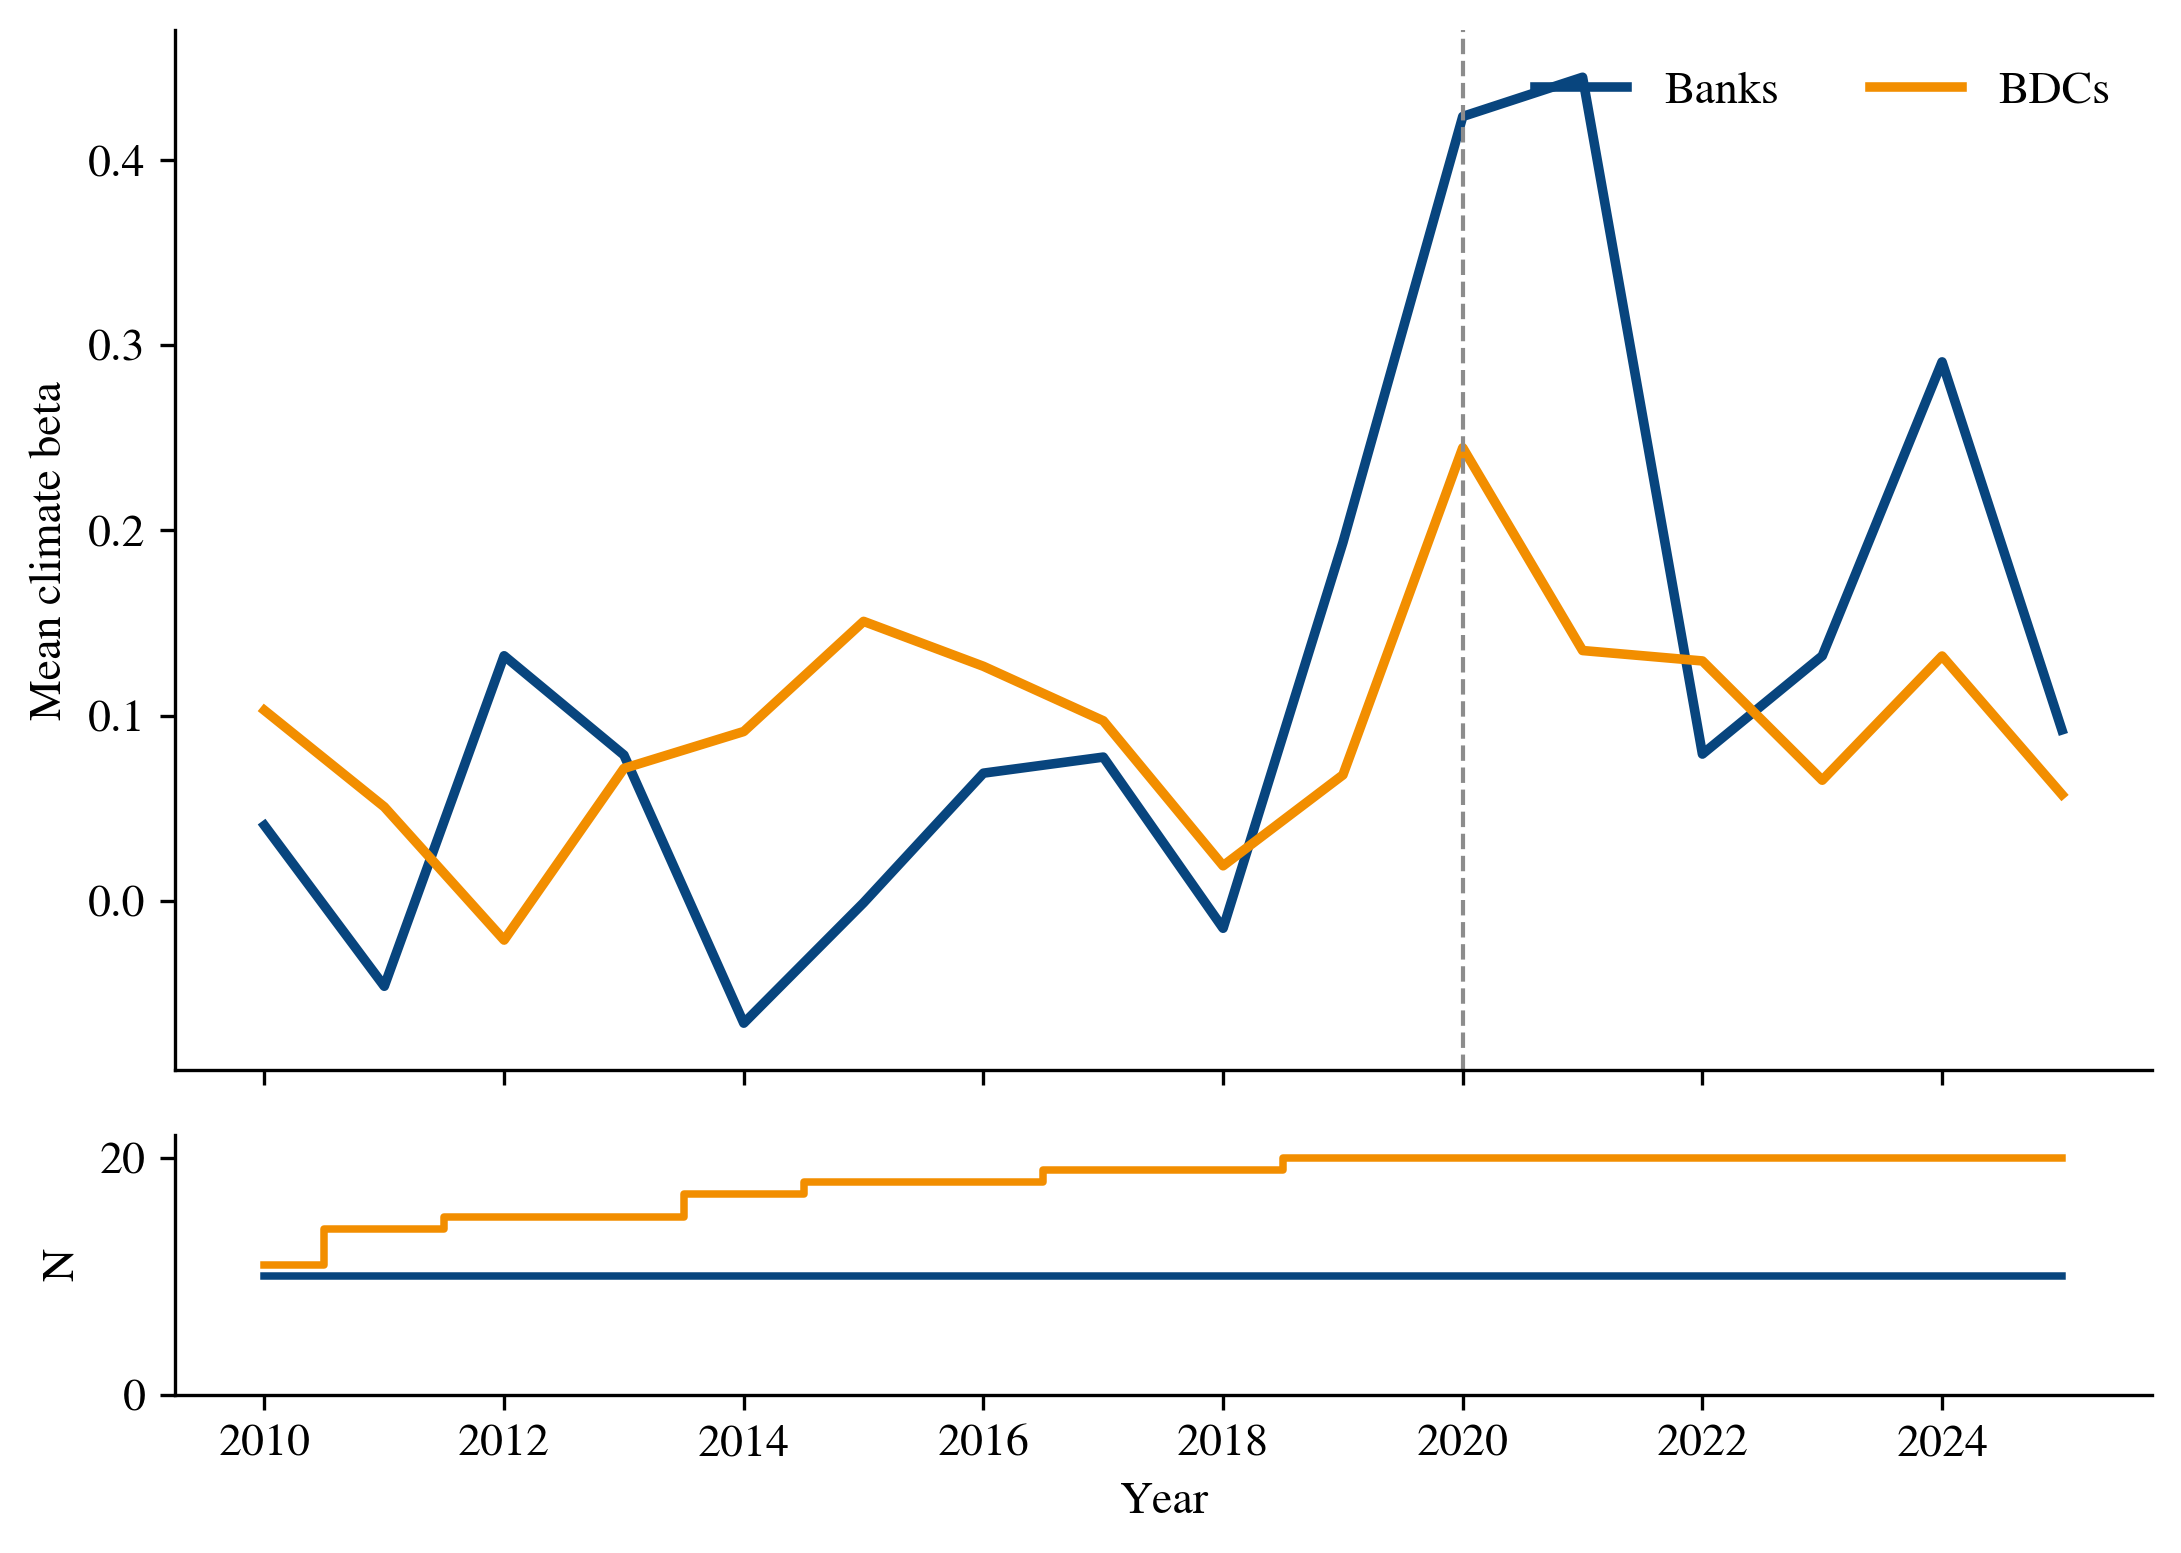
\includegraphics[width=0.95\textwidth]{../01_Bank_CRISK_Replication/Results/Figure_1_Aggregate_Climate_Beta.png}
\begin{minipage}{0.93\textwidth}
\footnotesize\textit{Notes:} The upper panel plots annual cross-sectional mean two-factor dynamic conditional climate beta; the lower panel reports the number of active institutions. The vertical line marks 2020. KOL is used through 14 December 2020 and the fixed USD top-five constituent return thereafter. Changes in the BDC series partly reflect entry and exit from the active sample.
\end{minipage}
\end{figure}

\clearpage
\begin{figure}[!h]
\centering
\caption{Top-Four Bank CRISK Around the 2020 Shock.\label{fig:bankcrisk}}
\vspace{0.06in}
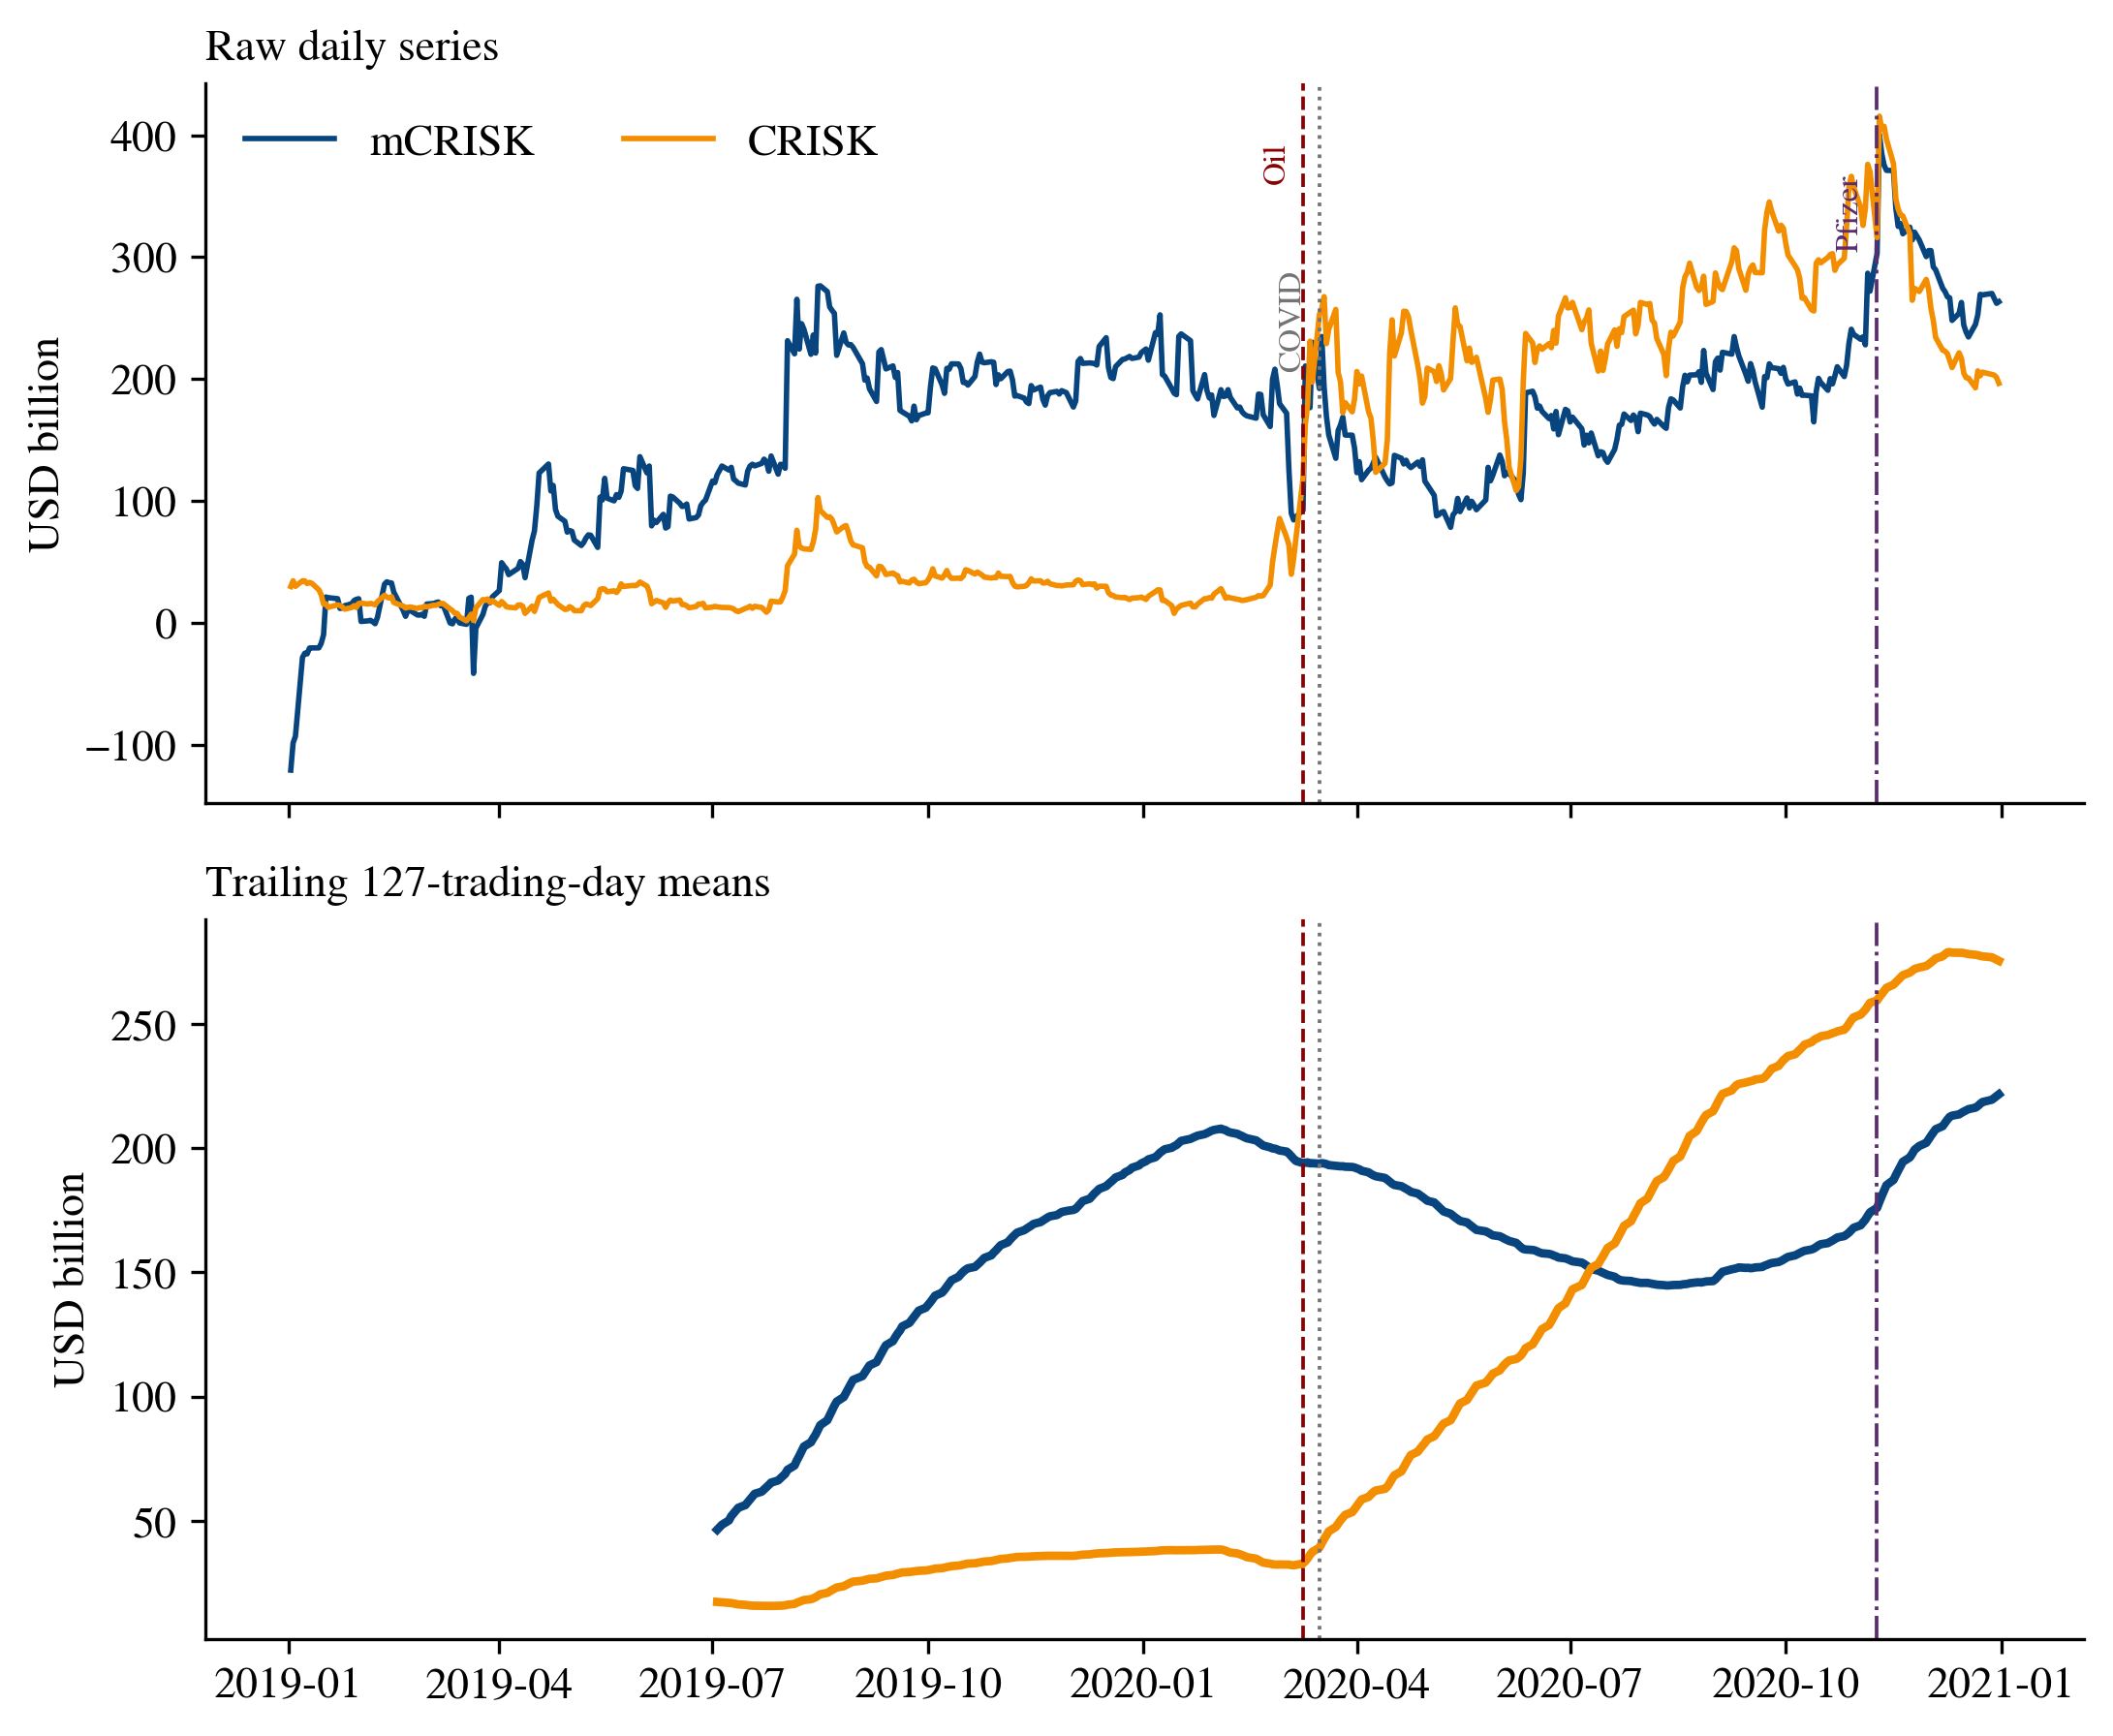
\includegraphics[width=0.95\textwidth]{../01_Bank_CRISK_Replication/Results/Figure_2_Top_Four_Bank_CRISK.png}
\begin{minipage}{0.93\textwidth}
\footnotesize\textit{Notes:} The upper panel reports raw daily series; the lower panel reports trailing 127-trading-day means for BAC, C, JPM, and WFC. Signed CRISK retains capital surpluses; positive CRISK truncates negative institution values at zero. Vertical markers identify the 9 March oil-price break, the 16 March COVID market dislocation, and the 9 November Pfizer--BioNTech announcement. Smoothing is shown separately so it cannot obscure event timing.
\end{minipage}
\end{figure}

\clearpage
\begin{figure}[!h]
\centering
\caption{Proximity to the Statutory Asset-Coverage Threshold.\label{fig:h3threshold}}
\vspace{0.06in}
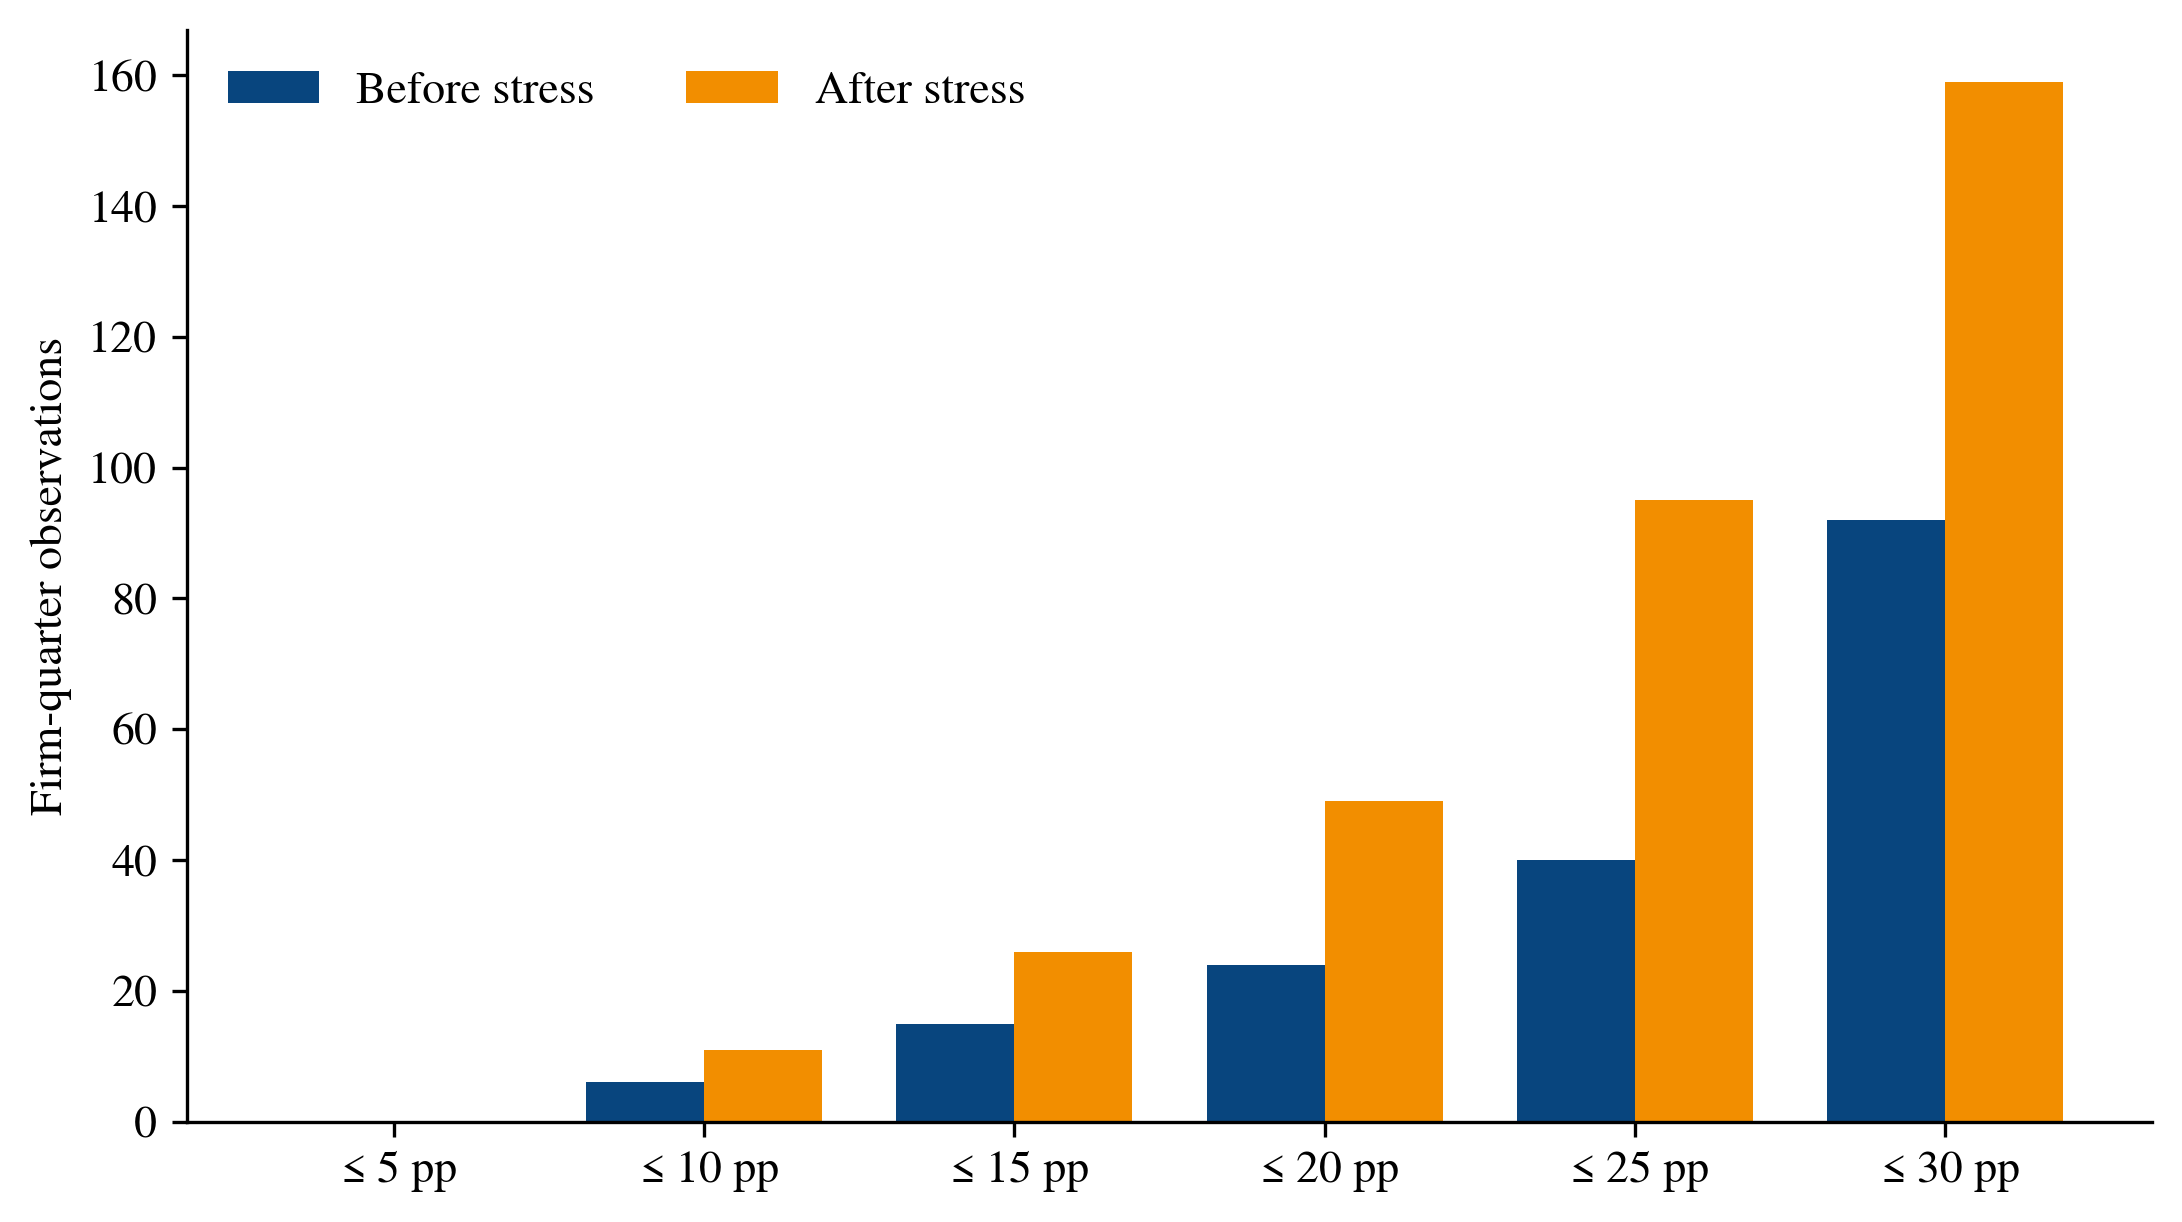
\includegraphics[width=0.95\textwidth]{../03_BDC_Asset_Coverage_Stress_Test/Results/Figure_7_Threshold_Proximity.png}
\begin{minipage}{0.93\textwidth}
\footnotesize\textit{Notes:} Bars count BDC-quarter observations within the indicated number of percentage points of the applicable 150- or 200-percent threshold. Categories are cumulative. No primary-scenario observation crosses the threshold.
\end{minipage}
\end{figure}

\end{document}
